\chapter{System Design and Implementation}\label{chapter:design_impl}

One of the main objectives in this thesis is the development of a prototype for a blockchain-based system that can operate as a decentralized index fund for investing cryptoassets passively. To this end, we design and develop a new \textit{DFAM token} that is composed of many underlying component tokens on the Ethereum blockchain. As such, the DFAM token acts as a portfolio with its price being determined by those of the constituting tokens and its circulating supply, thereby achieving portfolio diversification and broad market exposure. The developed DFAM token is a ERC-20 smart contract backed by another contract representing the index fund that facilitates the interactions with investors regarding the buying and selling of DFAM tokens. In this chapter, we first introduce the system architecture in section \ref{sec:sysarchitecture}. Then, in section \ref{sec:stakeholders}, the relevant stakeholders of the system will be presented. After that, we will discuss at length the external auxiliary systems relevant to our application in section \ref{sec:auxsystems} as well as inspect the core smart contracts and their functionalities in section \ref{sec:indextoken} and \ref{sec:indexfundcontract}. Then, section \ref{sec:oracleinfras} is concerned with the oracle infrastructure of the system and finally, we present a short discussion of the CLI client application in section \ref{sec:cli}.  

\section{System Architecture} \label{sec:sysarchitecture}

Overall, the proposed blockchain-based system is a DeFi application comprising both on-chain and off-chain components working in tandem with each other to perform the functionalities of the dApp. The on-chain components of the systems consist of three smart contracts in total, of which two \textit{core smart contracts} are responsible for the financial service of the application and the other one is an \textit{oracle contract}, which is part of the oracle infrastructure feeding data from the ITSA database into the core contracts. In addition, as the design of the system relies heavily on decentralized exchanges (DEXs), among which Uniswap V2 is the implementation of choice for the prototype, we also consider the Uniswap's smart contracts as part of the on-chain components in term of a required external auxiliary system that interfaces with our core smart contracts. On the other hand, the off-chain components involve a \textit{client application} and a \textit{oracle server} along with the external database from the ITSA for retrieving the classified token information. The client application is supposed to be used by the system's end-users, which we will also refer to as investors or shareholders from this point onward, to interact with the smart contracts. On the other end of the architecture, the oracle server is governed by the administrator of the dApp for the purpose of provisioning token data received from the ITSA into our smart contracts on the blockchain. In order to perform the portfolio composition selection process, the oracle server also receives price data sources from the Coingecko's price API. An overview of the entire system architecture is illustrated in Figure \ref{fig:sys_architecture}. 


% Figure

\begin{figure}
    \centering
  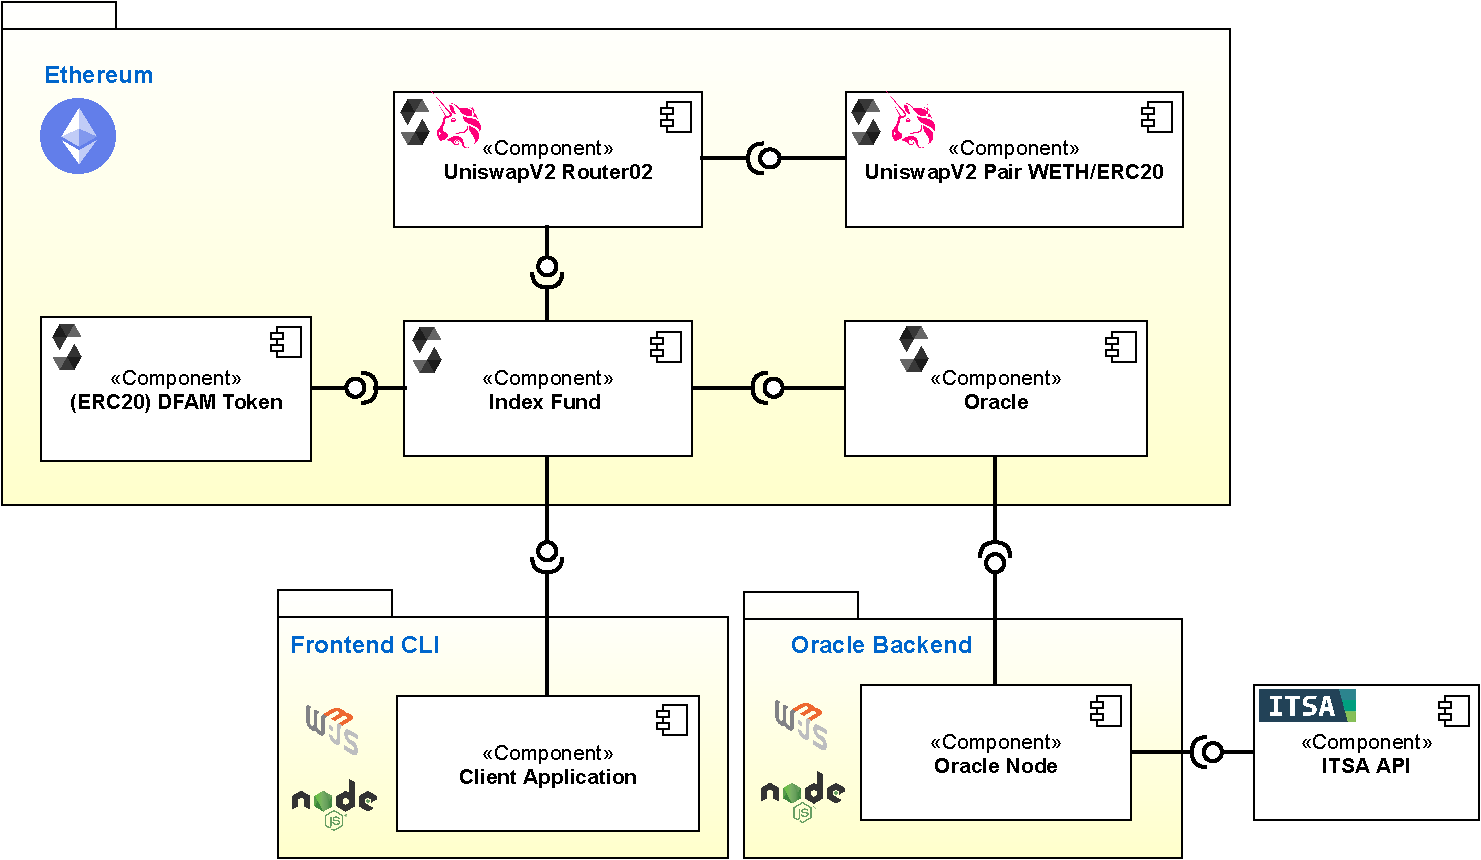
\includegraphics[width=\linewidth]{figures/system-architecture.pdf}
  \caption{System Architecture of the decentralized index fund application for Passive Asset Management}
  \label{fig:sys_architecture}
\end{figure}

In the following of this section, we will first present the relevant stakeholders of the system, then all the sub-systems and components will be closely examined in reference to the system overview depicted in Figure \ref{fig:sys_architecture}.


\section{Stakeholders of the System} \label{sec:stakeholders}

The concept of stakeholder in a software system is defined slightly differently in different software engineering literature sources. However, we relies on the definition in the well-cited book for software requirements by Karl Wiegers \cite{wiegers2013software}, in which stakeholder is defined as "an individual or group who is actively involved in the project, who is affected by the project, or who can influence its outcome". This definition is more or less in line with the well-know book from Pressman \cite{pressman2005software}, in which the roles of stakeholders in a software project are more clearly specified. Therefore, the specific stakeholders and their roles in the system can be described as follows.
% our work is a software project, but also a at the same time decentralized applications, whose on-chain components 

\begin{description}
	\item[Shareholder (Investor)] --- The end-users of the system are the Ethereum users investing in the DFAM token. Anyone whose EOA holds a non-zero balance of the DFAM token is considered the shareholder or the investor of the token. 

	\item[Liquidity Provider] --- We consider the liquidity providers from Uniswap (or from other DEXs in future versions of the system) are also the stakeholders of the system since they indirectly involve in the operation of the financial service of the dApp. Without their presence, there would be no liquidity for swapping between ETH and the underlying tokens (components) of the portfolio, therefore, they as well affects the functionality of the system to some extent.

	\item[The ITSA] ---  the ITSA is the data source provider for classified token information with their token API and the International Token Classification (ITC) framework \cite{itcDocs}.
	
% Currently, the first prototype of the system is developed by the Technical University of Munich as part of this thesis with the International Token Standardization Association (ITSA) being the project initiator, project manager as well as project advisor. In the upcoming versions, the system will possibly be further developed and maintained by the teams at the ITSA or other collaborators to realize our prototype into a real-world DeFi application.  Furthermore, another role of
	
% It should be noted that even though smart contract code may not be changed or bug-fixed after its deployment to the blockchain, future versions of our smart contracts can be developed and deployed as new contracts and their respective contract addresses can then be adapted to the other smart contracts and components interfacing with them within the system, thereby, achieving the upgradability of smart contracts.
	
% 	the ITSA will be responsible for the governance of the system during its actual operations, at least in the initial versions of this DeFi application. Although this might sound suspicious for a single party to control a decentralized application, many prominent cryptocurrency projects in the wild are still applying this model with the most notable examples including Aave, Compound and DDEX \cite{administratorKeysDefiProtocol}. However, this limitation might be cancelled in future versions with the use of a mechanism inspired from the concept of Decentralized Autonomous Organization (DAO) discussed in section \ref{???}. Last but not least, 
\end{description}




\section{External Auxiliary Systems} \label{sec:auxsystems}

This section intends to introduce the external systems that are not part of our development but their interactions are required to support the core functionalities of our DeFi application. We call them \textit{external auxiliary systems} and in Figure \ref{fig:sys_architecture} above, there are two such systems: \textit{Uniswap} and \textit{ITSA Database}. In the perspective of our system, the former comprises all the smart contracts deployed on the Ethereum blockchain by Uniswap , while the later is the off-chain database from the ITSA that can be accessed through an RESTful API. Both systems play an important role in our design and understanding them as well as their positions in our system will help with the explanation of the core system in the later sections of this chapter. In the following, the concept of Uniswap as well as its interactions with our prototype will be explored. Then, the token identification and classification frameworks of the ITSA will be characterized in sub-section \ref{subsec:itsa} along with the discussion of the ITSA's API, which provides the classified token information required for the portfolio of the decentralized index fund. 

\subsection{The Role of Uniswap in the System Prototype} 

Our system employs Uniswap as the DEX of choice for the trades between ETH received from investors and the collateralized underlying tokens of the portfolio. For this purpose, the \texttt{IndexFund} contract will use the Uniswap router as an interface to all the corresponding liquidity pools of the underlying components and WETH for all the swaps. When investors buy DFAM tokens, the ETH amount sent along for the purchase will be used by the \texttt{IndexFund} contract to swap for the underlying component tokens on Uniswap for the amounts proportional to the token prices at their respective liquidity pools. Reversely, when investors redeem their investments by returning their DFAM tokens back to \texttt{IndexFund}, a proportional amount of each underlying token will be swapped for ETH on Uniswap to refund the investors. As shown in Figure \ref{fig:sys_architecture}, the interaction between the \texttt{IndexFund} contract and \texttt{Uniswap Router V2} contract is the only connection between our DeFi application and the Uniswap's ecosystem. Therefore, all the trading traffic to Uniswap from our system will flow through this connection.

\subsubsection{Front-running Prevention}

One of the security issues that traders need to take into account is the front-running attack as mentioned in the Uniswap's documentation \cite{uniswapPricing}. In the event of a trader sending a transaction to perform token swapping at a particular liquidity pool on Uniswap, if malicious actors are aware of this transaction, they could perform a swap changing a large amount of pool reserves with a transaction that could be mined faster than that of the trader, e.g., with higher gas price specified. As a result, the swap of the trader would be executed at a possibly worse price than originally intended. Afterwards, the attacker can swap the amount of tokens received earlier back to the pool and effectively causing economic loss for the trader. It is worth noting that it is possible for the two transactions from the attacker to "sandwich" the target transaction of the trader within the same block.

For this reason, Uniswap recommends traders to inspect the price in advance and include into their swaps the amount of output token they expect to receive from the pool. When the real amount of tokens output does not satisfy the one specified by the trader, the transaction will be reverted, thereby, canceling the front-running attack. In our case, since the investors are the indirect traders of Uniswap pools, the purchase and redemption functionalities of \texttt{IndexFund} also require the possibility for including the expected amount of tokens received for each component as function parameters and incorporate them accordingly in the swapping requests sent to the Uniswap router. As such, our \texttt{IndexFund} contract directly inherits the mechanism of front-running prevention provided by Uniswap and helps investors avoid possible financial loss.


\subsection{ITSA Database} \label{subsec:itsa}

In addition to the Uniswap's smart contracts, another external auxiliary component in our system overview from Figure \ref{fig:sys_architecture} is the ITSA database, from which the classified token metadata can be retrieved for the inputs of the portfolio composition selection. Since we intend to have the portfolio follow a fixed token category, it is required that the tokens used as components of the portfolio must belong to that pre-specified category. However, the token space on Ethereum is constantly growing with new tokens and token metadata specified by the ERC20 standard does not allow to uniquely identify tokens and their categories. This causes certain difficulty for the selection of component tokens of the same category. 

\subsubsection{The ITC Framework of the ITSA}


The International Token Standardization Association is a non-profit organization with the goal of developing a universal framework for the identification, classification, and analysis of cryptographic tokens \cite{itsadefinition}. For these purposes, the ITSA collects, organizes and stores metadata of cryptocurrencies and tokens not only from the Ethereum blockchain, but also on other blockchains such as Bitcoin and Binance. In practice, token metadata such as names and symbols can be deliberately or accidentally duplicated, thereby causing misleading token identities. To address this issue, the ITSA proposes the International Token Identification Number (ITIN) framework, which is a standard of globally unique identification numbers that can be assign to tokens for more transparent and secure token identification. Furthermore, the ITSA also provide a flexible and extendable framework called the International Token Classification (ITC) so as to achieve effective classification of tokens into different dimensions and categories. Finally, the ITSA also features a token database called Tokenbase that provides qualitative and quantitative token data collected from various exchanges for the different purposes, especially token market analysis.


As the ITC frameworkof the ITSA can provide classified token metadata that can be used for the purpose of determining token categories, we rely on this framework for our portfolio selection process. From a technical point of view, the current version of the ITC classifies tokens with respect to a hierarchy with four dimension groups and six dimensions constituting the first two levels of the classification hierarchy. In the documentation of the ITC framework \cite{itcDocs}, the six dimensions are described as follows.

\begin{description}
    \item[Economic Purpose (EEP)] --- "The Dimension \textit{Economic Purpose} forms part of the Economic Dimensions, and provides information on the reason for a Token's creation as well as its intended use and functionality." 
    
    \item[Issuer Industry (EIN)] --- "The Dimension \textit{Issuer Industry} forms part of the Economic Dimensions, and provides information on the industry that the Issuer of a Token is active in."
    
    \item[Technological Setup (TTS)] --- "The Dimension \textit{Technological Setup} forms part of the Technological Dimensions, and provides information on the implementation and deployment style of a Token."
    
    \item[Legal Claim (LLC)] --- "The Dimension \textit{Legal Claim} forms part of the Legal Dimensions, and provides information on the rights that a Token provides its holder (Token Holder) with."
    
    \item[Issuer Type (LIT)] --- "The Dimension \textit{Issuer Type} forms part of the Legal Dimensions, and provides information on the nature of the Issuer of a Token."
    
    \item[Regulatory Status EU (REU)] --- "The Dimension \textit{Regulatory Status EU} forms part of the Regulatory Dimensions, and provides information on the potential classification of a Token according to the European Commission's proposal for a Regulation on Markets in Crypto Assets (MiCA, EU Regulation Proposal COM/2020/593 final)."

\end{description}

Each of the ITC dimension can be further divided into sub-levels that in turn can be split into even more specific sub-Level in the following order: Dimension Group (Level 1), Dimension (Level 2), Category (Level 3), Subcategory (Level 4), Class (Level 5), Subclass (Level 6), Group (Level 7), Subgroup (Level 8). The code of the higher, more general levels will be used to prefix the  the lower, more specific levels as can be seen from the first code letter of each of the six dimensions above with , for example, EEP and EIN belonging to the same Demension Group Ecomomic (E). However, current version of the ITC only reaches Level 6, thus, Group and Sub-group are being unused.

\subsubsection{The Portfolio Category of the System Prototype}

For the demonstrative purpose of our system prototype, we will assign a particular category of "Decentralized Lending, Saving and Asset Management"" to the token portfolio and additionally require that tokens retrieved from the ITSA must be ERC20-compliant. The tokens retrieved from ITSA's API should have the ITC codes of \textbf{EIN06DF02} and \textbf{TTS42ET01} in order to be a candidate component for the token portfolio. The following breakdown will explain the meaning of the code according the ITC framework documentation \cite{itcDocs} and the prefix rule discussed above.

\begin{itemize}
    \item \textbf{TTS42ET01} --- \textbf{T} (Dimension Group \textit{Technological}), \textbf{TS} (Dimension \textit{Technological Setup}), \textbf{42} (Category \textit{Application Layer Token}), \textbf{ET} (Subcategory \textit{Ethereum Application Layer Token}), 01 (Class \textit{Ethereum ERC-20 Standard Token})
    
    \item \textbf{EIN06DF02} --- \textbf{E} (Dimension Group \textit{Economic}), \textbf{IN} (Dimension \textit{Issuer Industry}), \textbf{06} (Category \textit{Finance and Insurance}), \textbf{DF} (Subcategory \textit{Decentralized Finance (DeFi)}), \textbf{02} (Class \textit{Decentralized Lending, Saving and Asset Management})
\end{itemize}

Therefore, when our system queries the token metadata through the ITSA's RESTful API during the portfolio section process, the GET request will contain these two ITC codes so that ITSA database could perform the filtering and return only the tokens that match the two requirements. With the help of the ITC framework, our decentralized index fund can effectively allow investing into tokens in a specific category of investors' interest.



\section{The DFAM Token Contract} \label{sec:indextoken}

The smart contract for defining the DFAM token will closely follow the ERC20 token standard due to the benefits of ERC20 that have been discussed in section \ref{subsec:tokenerc20}. Generally, ERC20-compliant tokens are widely supported by most decentralized applications  on Ethereum, especially by the most well-known CEXs and DEXs such as Binance, Uniswap and SushiSwap. Moreover, a variety of crypto-wallets including MyEtherWallet (MEW) and MetaMask provide built-in support for the ERC20-compliant tokens with automatic recognization and integration of the ERC20 interface.

Essentially, the ERC20 standard only serves as a token interface specifying a set of functions a fungible token should support, thus, developers of an ERC20-compliant token are responsible for the implementation of the specified functions into a smart contract. Nonetheless, since ERC20 is unarguably one of the most widely used standard in Ethereum, there are many third-party libraries offering deployable ERC20 contract scripts pre-composed out of the box and one of such libraries is OpenZeppelin, whose ERC20 contract script is our preferred ERC20 implementation for the DFAM token. The use of a pre-composed ERC20 smart contract from a library not only cancels the potential of introducing bugs by developers, especially with respect to such important code for the essential functions of a token smart contract, but also helps incorporate the mitigations of known security issues discovered by the community during the practical use of the standard. An example of such mitigations is the two non-standard \texttt{decreaseAllowance} and \texttt{increaseAllowance} functions that have been integrated into the ERC20 smart contract of OpenZeppelin to address an attack vector related to the \texttt{approve} and \texttt{transferFrom} functions of ERC20. This attack vector is comprehensively described by Vladimirov and Khovratovich in their public announcement \cite{vladimirov2018erc20}. In Listing \ref{lst:erc20attack}, the implementation of the \texttt{decreaseAllowance} and \texttt{increaseAllowance} functions in Solidity can be explored . \\


\begin{lstlisting}[language=Solidity, label={lst:erc20attack}, captionpos=b, caption={Solidity code of the \texttt{decreaseAllowance} and \texttt{increaseAllowance} functions for ERC20 from OpenZeppelin to mitigate the attack vector related to the \texttt{approve} function described in \cite{vladimirov2018erc20}\\}]
...
function increaseAllowance(address spender, uint256 addedValue) public virtual 
    returns (bool) {
        _approve(_msgSender(), spender, _allowances[_msgSender()][spender] + addedValue);
        return true;
}

function decreaseAllowance(address spender, uint256 subtractedValue) public virtual 
    returns (bool) {
        uint256 currentAllowance = _allowances[_msgSender()][spender];
        require(currentAllowance >= subtractedValue, "ERC20: decreased allowance below zero");
        _approve(_msgSender(), spender, currentAllowance - subtractedValue);
        return true;
}
...
\end{lstlisting}


As shown in Listing \ref{lst:erc20attack}, the \texttt{increaseAllowance} and \texttt{decreaseAllowance} functions enable explicitly incrementing and decrementing the allowance, respectively, instead of replacing the old allowance with a new allowance as with the conventional \texttt{approve} function from the ERC20. In short, the increment or decrement of allowance should be used instead of replacement of allowance. Besides these two non-standard functions, the ERC20 contract from OpenZeppelin also offers two additional internal functions called \texttt{\_mint} and \texttt{\_burn}, which are used to mint and burn tokens, respectively. Since this ERC20 smart contract is supposed to be inherited from a custom contract created by the users of the library, these internal functions are not used anywhere in the ERC20 contract and are open for a derived contract to decide whether to offer their respective functionalities or not. Thus, the \texttt{\_mint} and \texttt{\_burn} functions  are also annotated as \texttt{virtual} functions. Furthermore, this ERC20 contract also includes an empty hook, which is also marked as \texttt{internal} and \texttt{virtual} and is supposed to be implemented by the library user as a supplementary function for \texttt{\_mint} and \texttt{\_burn} to execute additional business logic before tokens are minted or burnt.


\begin{lstlisting}[language=Solidity, label={lst:indextokencontract}, captionpos=b, caption={Solidity code of the \texttt{DFAM} smart contract\\}]
//SPDX-License-Identifier: MIT
pragma solidity ^0.8.0;

import "@openzeppelin/contracts/access/Ownable.sol";
import "@openzeppelin/contracts/token/ERC20/ERC20.sol";

contract DFAM is ERC20, Ownable {
    constructor() ERC20("DeFi Asset Management Index", "DFAM") {  }


    function mint(address _to, uint256 _amount) onlyOwner external returns (bool) {
        _mint(_to, _amount);
        return true;
    }

    function burn(uint256 _amount) external returns (bool) {
        // can only burn the tokens that the caller owns
        _burn(msg.sender, _amount);
        return true;
    }
}
\end{lstlisting}

By inheriting from the OpenZeppelin's ERC20 contract, the smart contract defining our DFAM token is rather short and is named as \texttt{DFAM}. The entire code of the \texttt{DFAM} contract is shown in Listing \ref{lst:indextokencontract}. In addition, the \texttt{DFAM} contract also inherits from the abstract contract \texttt{Ownable}, which allows the account deploying the \texttt{DFAM} contract to become the contract owner. As a result, the \texttt{onlyOwner} modifier declared in the \texttt{Ownable} contract can be used to protect the external function \texttt{mint} from being executed by unauthorized accounts other than the owner. The idea of having an owner is to prevent the public from minting new tokens out of thin air using the \texttt{mint} function from lines 11 to 14. However, the owner and also the deployer of the \texttt{DFAM} contract is in fact the \texttt{IndexFund} contract, which is also shown in Figure \ref{fig:sys_architecture} and will be discussed next in section \ref{sec:indexfundcontract}. Consequently, investors have to purchase DFAM tokens through the \texttt{IndexFund} contract since this is the only way to add new tokens into circulation. The logic of the \texttt{mint} function is also simple. It accepts the address of the token receiving account as the first parameter (\texttt{\_to}) and the amount of tokens to mint as the second one (\texttt{\_amount}). Then, the internal \texttt{\_mint} function from the \texttt{ERC20} contract is called to create new tokens and transfer them to the account at the address \texttt{\_to}. Finally, the function signifies that the minting completes successfully by returning \texttt{true} so that it is possible to place the \texttt{mint} function inside a \texttt{require} function for validating the completion of the process. 


The constructor of \texttt{DFAM} in line 8 has no parameters and is there only for the purpose of calling the constructor of the \texttt{ERC20} contract with the name of the token being \texttt{DeFi Asset Management Index} and the symbol being \texttt{DFAM}. The DFAM token will have the \texttt{decimals} of \texttt{18}, therefore, the smallest denomination of the token is worth $10^{-18}$ \texttt{DFAM}. It is also important to note that the token supply after the deployment of \texttt{DFAM} is zero since the supply should only be incremented when the DFAM tokens are purchased and decremented when investors redeem their investments by selling DFAM tokens back to the index fund. In this manner, the total token supply is in fact dynamic.
Finally, we also support the burning of DFAM tokens with the \texttt{burn} function from line 16 to 20 in Listing \ref{lst:indextokencontract} and anyone can burn their DFAM tokens without any restrictions. Indeed, token shareholders can always burn their tokens by sending them to the zero address (\texttt{address(0x0)}). However, the circulating supply will not be reduced by this burning method and therefore, the DFAM price dependent on the token supply will not be affected. For this reason, we also provide the \texttt{burn} function as a means to burn tokens in an organized manner for a correct reduction of the total supply in favor of the DFAM price calculation.


\section{The Index Fund Contract} \label{sec:indexfundcontract}

As shown in Figure \ref{fig:sys_architecture} for the system architecture, the \texttt{IndexFund} smart contract is effectively the central point of the application considering the direct interactions it has with other components. On the blockchain, it controls the minting of DFAM tokens from the \texttt{DFAM} contract and interacts with the Uniswap router to swap between ETH and the component tokens of the portfolio. In addition, it also acts as the client of the oracle contract for the token data from the ITSA database as well as being the entry point for the end-users, who use the off-chain client component to access the financial service offered by this smart contract. As a result, the \texttt{IndexFund} contract plays a crucial role in this DeFi application and it is indeed responsible for main business logic of the application. 
In the next pages of this section about the \texttt{IndexFund} smart contract, we will discuss the structure and the functionalities of this contract separate sub-sections. Thereby, its interactions with different other components of the system.

\subsection{Inheritance Structure}

The \texttt{IndexFund} smart contract inherits directly from two abstract smart contracts \texttt{Fund} and \texttt{TimeLock}. These parent contracts all serve as means of code reduction and organization for the ease of development, however, each of them also provides contract \texttt{IndexFund} with additional features that can be described as follows.

\begin{description}
  \item[The abstract contract \texttt{Fund}] ---  As a general index fund contract has a portfolio comprising component tokens in a specific ITC category from the ITSA, it is likely the case that in the future, many index fund contracts with different portfolio categories will be developed and deployed to allow investments in different index tokens (resembling DFAM) of various categories. Therefore, the contract \texttt{Fund} serves as a common template for any derived index fund contracts to follow. As such, this abstract contract holds the state variables that every index fund should have such as the portfolio information. In addition, it also specifies the signature of all essential functions that should be implemented by a derived contract with examples being \texttt{buy} and \texttt{sell} to support the buying and selling of DFAM tokens respectively. Finally, all the relevant events that should be emitted during the operations of an index fund contract are as well defined in this contract.
  
  \item[The abstract contract \texttt{TimeLock}] --- This contract offers the feature of locking the invocation of specific functions in \texttt{IndexFund} for a certain period of time. In our case, \texttt{updatePortfolio} and \texttt{rebalance} are the two functions that have to be time-locked for two days before any of their actual executions. Since these two functions directly modify the component balances that \texttt{IndexFund} holds and therefore, affecting the profits of investors, the purpose of locking them  for two days before they are allowed to be invoked is to give the investors, who disagree with the next portfolio update or rebalancing sufficient time to redeem their investments and return their DFAM tokens back to \texttt{IndexFund}. This behavior will be explored more closely in the respective sections \ref{subsec:updateportfolio} and \ref{subsec:reblance}.
  
%   \item[The abstract contract \texttt{Ownable}] --- Certain functions in the smart contract \texttt{IndexFund} are restricted to be executed only by its administrator(administrator). This abstract contract is pre-composed from OpenZeppelin to allow a derived smart contract to apply such restriction with the use of the function modifier \texttt{onlyOwner}. When \texttt{IndexFund} is deployed, the message sender is set as its owner and therefore, the administrator of \texttt{IndexFund} is bydefault the contract deployer. However, the administrator can be changed through the function \texttt{transferOwnership} in \texttt{Ownable} at any time by the administrator themselves. 
  
\end{description}

\subsection{Storage Data and Function Modifiers}
Due to the frequent interactions with the smart contracts \texttt{DFAM}, \texttt{Oracle} and the Uniswap router contract as shown in Figure \ref{fig:sys_architecture}, the \texttt{IndexFund} contract will hold the addresses of those smart contracts in its storage as public state variables, thereby, allowing any interested parties such as shareholders and potential investors to inspect and validate them. Besides, the address of  the Wrapped Ether token (\texttt{WETH}) is also stored in the storage since this address will be used in almost all the functions that are related to the swapping between ETH and component tokens. It is important to note that these four address state variables (\texttt{DFAM},  \texttt{Oracle}, \texttt{WETH} and the Uniswap router are set as \texttt{immutable}, and therefore, cannot be changed during the life-time of \texttt{IndexFund}) after their assignments during the contract construction time as per the design in this initial version of our DeFi application.

Additionally, there are another two state variables that store the important portfolio information in the abstract \texttt{Fund} contract, from which the \texttt{IndexFund} contract is derived. The one variable is \texttt{components}, which is a string array storing the symbols of the component tokens in the portfolio, and the other is \texttt{portfolio}, which is a mapping from component symbols of string type to the addresses of the underlying component tokens. As such, in order to obtain the address of a particular component token from \texttt{portfolio}, its symbol is required as the input into this mapping and can first be selected from the \texttt{components} array. 

By inheriting from the abstract contract \texttt{TimeLock}, the \texttt{IndexFund} contract also inherits two public state variables related to the function time-locking feature. One is a constant variable \texttt{TIMELOCK} specifying the period of \textit{two days} for each locking and the other is a mapping from function identifiers to the due lock-time of the respective functions.

At its construction time, the \texttt{IndexFund} contract will receive the data to fill its state variables. Specifically, the constructor of \texttt{IndexFund} receives as its parameters the address of the Uniswap router contract and the \texttt{Oracle} contract as well as two arrays for the symbols and addresses of the portfolio components. Also during the construction time of \texttt{IndexFund}, it will deploy the \texttt{DFAM} contract, thus, obtain the address returned after the deployment and become the owner of \texttt{DFAM}. The address of \texttt{WETH} is, however, acquired through a message call to the Uniswap router.

There is also the function modifier \texttt{onlyOracle} used by \texttt{IndexFund} to restrict the invocation of the functions modifying the portfolio. The modifier ensures that only the \texttt{Oracle} contract can invoke the functions that update and rebalance the portfolio. In our design, any functions annotated with the \texttt{onlyOracle} modifier in the \texttt{IndexFund} contract will always require to be time-locked for two days before their invocation is permitted. This guarantee that important changes to our decentralized index fund by a governing entity such as the \texttt{Oracle} contract are always restricted by locking time, thereby, investors can be assured about the safety their investments. A summary of all the public state variables as well as function modifiers in the \texttt{IndexFund} contract can be seen in Table \ref{tab:indexfundstatevars} below.

\begin{longtable}{p{.15\textwidth}p{.3\textwidth}p{.45\textwidth}}
    \toprule 
    \textbf{Name} & \textbf{Type} & \textbf{Description} \\
    \midrule
    \texttt{router} & \texttt{address immutable} & Address of the Uniswap router contract \\
    \texttt{weth} & \texttt{address immutable} & Address of the Wrapped ETH contract \\
    \texttt{oracle} & \texttt{address immutable} & Address of the \texttt{Oracle} contract \\
    \texttt{indexToken} & \texttt{address immutable} & Address of the \texttt{DFAM} contract \\
    \texttt{components} & \texttt{string[]} & Array of symbols of the component tokens \\
    \texttt{portfolio} & \vtop{\hbox{\strut \texttt{mapping}}\hbox{\strut \texttt{(string => address)}}} & Mapping from symbols to addresses of the component tokens \\
    \texttt{TIMELOCK} & \texttt{uint256 constant} & Constant for lock time of \texttt{2 days} \\
    \texttt{Functions} & \texttt{enum} & Enum as function identifiers \\
    \texttt{timelock} & \vtop{\hbox{\strut \texttt{mapping}} \hbox{\strut \texttt{(Functions => uint256)}}} & Mapping from function identifier to their current lock time \\
    \texttt{onlyOracle} & \texttt{modifier} & Function modifier to restrict function execution to only the \texttt{Oracle} contract \\
    \texttt{onlySupported} & \texttt{modifier} & Function modifier to allow only supported functions specified in the \texttt{Functions enum} can be time-locked  \\
    \texttt{notLocked} & \texttt{modifier} & Function modifier to ensure that time-locked functions can only be executed when their lock time is due \\
    \bottomrule
    \caption{\label{tab:indexfundstatevars} Public state variables and modifiers of \texttt{IndexFund}}
\end{longtable}


\begin{figure}
    \centering
  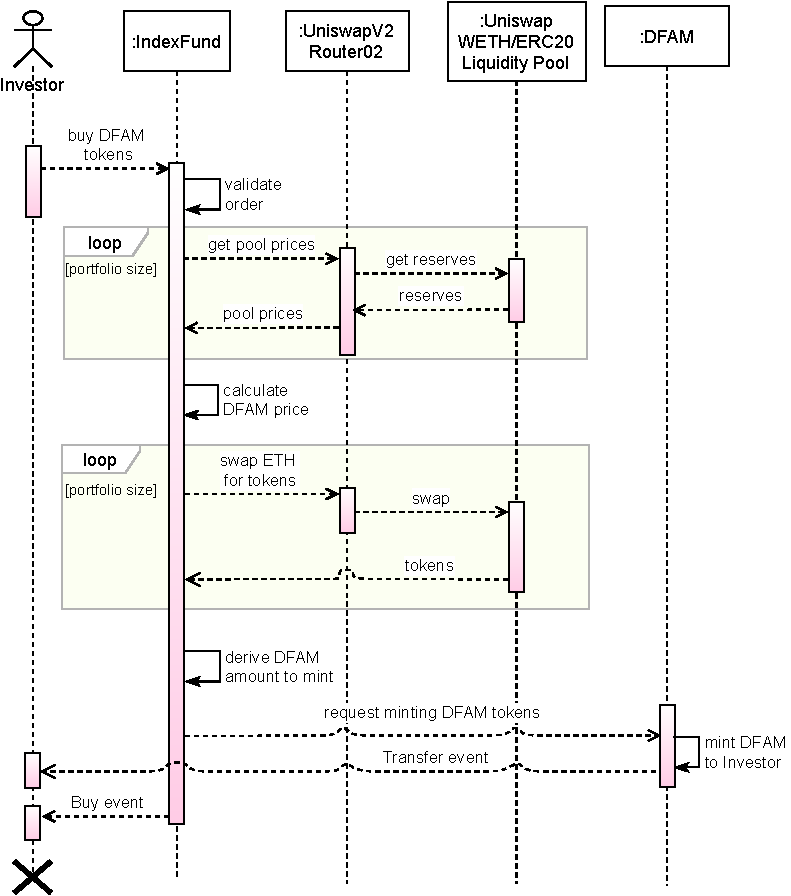
\includegraphics[width=\linewidth]{figures/purchase-seq.pdf}
  \caption{DFAM token's purchasing workflow}
  \label{fig:seq_purchase}
\end{figure}

\subsection{Handling of Investments in Index Fund} \label{subsec:handlinginvestment}

The main functionality that the \texttt{IndexFund} contract offers to the investors is the ability to purchase DFAM tokens as a means to invest into the underlying component crypto-tokens. The general idea is that investors send ETH as investment capital to the \texttt{IndexFund} contract in return for a proportional amount of DFAM tokens representing investors' share in our index fund. Then, the invested amount of ETH is used to swap for the underlying tokens of the portfolio on the decentralized exchange Uniswap. The DFAM price is averaged from the price of the underlying component tokens and the current circulating supply in order to achieve diversified market exposure and less price fluctuation. For reference, the sequence diagram in Figure \ref{fig:seq_purchase} illustrates the entire workflow for the process of investing in DFAM tokens with the interactions between the investors, the \texttt{IndexFund} contract and Uniswap router contract. Nonetheless, this process can be more thoroughly explained step by step in the perspective of the \texttt{IndexFund} contract as follows.

\begin{description}
  \item[Step 1: Validate purchase order] --- For the purpose of settling investments in DFAM tokens, the \texttt{IndexFund} contract provides an external function called \texttt{buy}, which is also a \texttt{payable} function accepting an ETH amount sent in the calling transaction as the investment capital. For the \texttt{buy} function to be executed, the transactions calling this function are required to holds a positive amount of ETH, meaning a \texttt{msg.value} greater than zero. Moreover, as part of the front-running prevention mechanism, investors can also to pass in the \texttt{buy} function a parameter specifying the minimum amounts of component tokens that \texttt{IndexFund} should be receiving from Uniswap.

  \item[Step 2: Calculate current DFAM price] ---  Since the DFAM price is influenced by the amount of the underlying component tokens that the \texttt{IndexFund} holds, the current DFAM price should be stored before the swapping from ETH to component tokens is executed on Uniswap. Let $P_{DFAM}$ be the DFAM price, then $P_{DFAM}$ can be calculated using the one of the formulas in Equation \ref{eq:bootstrap_calc} or Equation \ref{eq:price_calc} depending on whether the current DFAM Token supply is zero or not.
  

  \item[Step 3: Swap ETH for component tokens] --- The \texttt{buy} function can now swap the amount of ETH received from the investor for the underlying tokens of the portfolio on Uniswap through the Uniswap router contract. As sophisticated portfolio allocation is not the focus of our prototype, for simplicity, the sum of ETH received will be uniformly distributed among the each component token and the same amount of ETH will be used for each component to swap for an equivalent token amount at their respective liquidity pools. For example, if the portfolio comprises 10 component tokens and the investment capital sent to the \texttt{buy} function is 10 ETH, then, for each component in the portfolio, the \texttt{buy} function will swap 1 ETH for an equivalent amount of that component token. As a result, there will be 10 swaps at 10 respective \texttt{WETH/<COMPONENT$_i$>} liquidity pools. It should be noted that the amounts of component tokens received from the swaps are held by the \texttt{IndexFund} contract and not by the investor, who will, however, receive an DFAM Token amount equivalent to their investment in the last step of the workflow.
  
  \item[Step 4: Derive the amount DFAM tokens to be minted] \label{step:step4purchase} --- Based on the total component token amounts received from the swaps, the Net Asset Value (NAV) in ETH of the current purchase can be calculated. The NAV is the equivalent amount of ETH the \texttt{IndexFund} contract receives when it were to swap those component token amounts back to Uniswap. Therefore, NAV effectively represents the actual ETH value of the current underlying assets. It is also important to note that the ETH NAV is less than the investment capital (\texttt{msg.value}) originally sent by the investor due to the 0.3\% fee of Uniswap. Ultimately, the amount of DFAM tokens that should be minted for the investor is derived based on the ETH NAV of the purchase and the $P_{idex}$ from in Step 2 using the formula in the Equation \ref{eq:minting}.

\begin{equation} \label{eq:minting}
  amount_{minted} = \frac{NAV_{purchase} }{P_{DFAM}} 
\end{equation}
  
  \item[Step 5: Mint new DFAM tokens to investors] --- In exchange for the capital invested, investors will receive from the \texttt{IndexFund} contract a proportional amount of DFAM tokens derived in Step 4. Since \texttt{IndexFund} is the owner of the \texttt{DFAM} contract, it is the only account that has the privilege to mint new DFAM tokens due to the \texttt{onlyOwner} function modifier annotated on the \texttt{mint} function as shown in Listing \ref{lst:indextokencontract}. At the end, a \texttt{Buy} event is emitted to signify the success of the purchase with information about investor's wallet address, amount of tokens minted and the DFAM price used for the purchase. From this point onward, the investor becomes the \textit{shareholder} of the DFAM Token with their DFAM tokens proving their shares in the decentralized index fund.

\end{description}


It is important to note that the order of Step 2 and 3 above are crucial. In theory, it is possible to execute the swaps on Uniswap before the calculation of the current DFAM price, however, this would lead to a wrong derivation of DFAM token amount because the DFAM price depends on the amount of the underlying component tokens that the index fund is holding. 

Among all the steps above of the investment workflow, the swapping of ETH for component tokens is a most long-running process involving significantly many number of message calls and operations executed at different liquidity pools on Uniswap, therefore, it has the highest potential to be interrupted, e.g., due to out of gas or other errors occurring in the middle of the swapping process. Even though the EVM will revert the Ethereum world state back to the state prior to the execution of the transaction if the purchase fails to complete and the investor will not lose their investment capital, the total gas used could be, however, significant for the investor. Therefore, transactions should set a \texttt{startGas} high enough to cover the complete execution. As a matter of fact, the more component tokens in the portfolio, the higher the gas needed to successfully run the \texttt{buy} function due to the looping through multiple liquidity pools to execute the swaps.  

\subsection{Handling of Investment Redemption}

Generally speaking, an DFAM token act as a \textit{meta-token} comprising a set of underlying component tokens with their respective individual NAV contributing to the total NAV of the index fund. As such, when investors purchase an DFAM token, they in fact indirectly purchase the underlying component tokens from Uniswap and also, indirectly own them through our index fund. Although the balances of the underlying component tokens are directly owned by the \texttt{IndexFund} contract, every shareholder can at anytime prove their shares in the fund and redeem their investments through their DFAM tokens they own as it is always possible for shareholders to execute investment redemption by selling their DFAM tokens back to the \texttt{IndexFund} contract and receive the corresponding payout in ETH through the external function \texttt{sell} provided he \texttt{IndexFund} contract. The work flow of investment redemption follows a reversed direction compared to purchasing workflow above and is executed as follows.


\begin{description}
  \item[Step 1: Approving DFAM tokens to \texttt{IndexFund} by shareholders] --- When shareholders intend to sell back a certain amount of DFAM tokens to the \texttt{IndexFund} contract in exchange for ETH, they must first allow the \texttt{IndexFund} contract to withdraw that amount of DFAM tokens from them by calling the ERC20's \texttt{approve} function in the \texttt{DFAM} smart contract.

  \item[Step 2: Validate redemption orders] --- After approving the withdrawal of DFAM tokens, shareholders can now call the \texttt{sell} function of the \texttt{IndexFund} contract with a parameter specifying the actual amount of DFAM tokens they wish to sell. At this point, the \texttt{sell} function will check whether the allowance the \texttt{IndexFund} contract received from the shareholder in the previous step is greater than or equal to the amount specified in the parameter or not. The check can be accomplished with a message call to the \texttt{allowance} function in the \texttt{DFAM} contract. If sufficient amount of DFAM tokens is allowed, the function will proceed further, otherwise, an error will be thrown with a message stating that the allowance of DFAM token amount is not sufficient. Also, as with the \texttt{buy} function, it is possible for investors to pass to the \texttt{sell} function an array containing the expected amounts of ETH received from Uniswap for each component token.
  
  \item[Step 3: Transferring DFAM tokens to the \texttt{IndexFund} contract] --- With the amount of DFAM tokens approved by the shareholder in Step 1, the \texttt{IndexFund} contract can now transfer that DFAM token amount to itself and temporarily own these tokens during the execution of the workflow. 
  
  \item[Step 4: Calculate current DFAM price] --- This step is performed in the same manner as Step 2 of the purchasing workflow presented in section \ref{subsec:handlinginvestment} to receive $P_{DFAM}$.

  \item[Step 5: Deriving the NAV reduction of each component token] --- Since the investment capital was evenly distributed to each component to swap fro ETH during the purchasing process. Therefore, we perform a reverse calculation in this step and expect each component should uniformly contribute to the sum of ETH that is eventually returned to the investor. Thus, the current NAV of each component should be deduced by the same amount and the reduction amount is calculated with the formula in Equation \ref{eq:navreduced}, where $NAV_{reduced}$ is the amount of ETH each component contributes to the swap in the next step, $amount_{sold}$ is the DFAM token amount the investor is selling and $n$ is the number of component tokens in the portfolio or the portfolio size. 
  
\begin{equation} \label{eq:navreduced}
NAV_{reduced} = \frac{amount_{sold} \cdot P_{DFAM}}{n} 
\end{equation}
  

\item[Step 6: Swapping component tokens for ETH] --- In this step, the \texttt{DFAM} contract executes the swaps from the component tokens to ETH at their respective \texttt{WETH/<COMPONENT$_i$>} liquidity pools. The ETH amount input into each pool is the $NAV_{reduced}$ derived in Step 5. Therefore, after the swaps, the NAV of each component token will be decreased by $NAV_{reduced}$. The total amount of ETH received from Uniswap pools, which equals $n \cdot NAV_{reduced}$, will be sent directly from Uniswap's pools to the wallet of the investor.


\item[Step 7: Burn the returned DFAM Tokens] --- Finally, the \texttt{IndexFund} contract invokes the \texttt{burn} function in the \texttt{DFAM} contract to burn the amount of DFAM tokens returned by the investor in Step 3, thereby, decreasing the total supply of DFAM tokens.

\end{description}

For the sake of simplicity within the scope of a system prototype, we use the uniform distribution for the allocation of component tokens during both the investment and redemption processes. However, future versions of the application may use more sophisticated strategies for component allocation, which will require expertise in finance and therefore, these two processes can become much more complicated.

\subsection{Calculation of DFAM Token Price} \label{subsec:indexprice}

One of the main goals of the DFAMI Token is to mitigate the risk of abruptly fluctuating price in cryptocurrency investment by providing the investors diversified market exposure with an DFAM token comprising many different underlying tokens. As the DFAM price is directly aggregated from the prices of the underlying component tokens, the abrupt price fluctuation of each individual token only partially affects the DFAM price if the other component prices in the portfolio still remain stable. As such, investors can manage their investments in the component tokens passively and indirectly through our DFAM token without concerning about the unexpected price fluctuations that can potentially cause significant losses. In principle, the DFAM price also depends on the the circulating supply of DFAM token and the total NAV held by the \texttt{IndexFund} contract. The following formula shows how the DFAM price with a portfolio of $n$ component tokens is calculated:

\begin{equation} \label{eq:price_calc}
P_{DFAM} = \frac{b_1 p_1 + b_2 p_2 + \ldots + b_n p_n}{S} = \frac{NAV_1 + NAV_2 + \ldots + NAV_n}{S}
\end{equation}

where $P_{DFAM}$ denotes the DFAM price, $S$ is the circulating supply of DFAM tokens, $b_i$ indicates the balance of component token $i$ that the \texttt{IndexFund} contract is holding, $p_i$ expresses the price of component token $i$ in the respective \texttt{WETH/<COMPONENT$_i$>} pool on Uniswap, and $NAV_i$ represents the net asset value of component token $i$ that the \texttt{IndexFund} contract has if the entire $b_i$ is swapped at price $p_i$ on Uniswap.

In the \texttt{IndexFund} contract, the formula in Equation \ref{eq:price_calc} is encoded in the public function \texttt{getIndexPrice}, which calls the \texttt{getAmountsOut} function of Uniswap router to retrieve the component token prices $p_i$ as well as contacts the respective component token contracts for the balances $b_i$. Furthermore, the current DFAM total supply $S$ is queried by calling the function \texttt{totalSupply} in the smart contract \texttt{DFAM}. As a result, the calculation of the DFAM price requires a significant number of message calls for it to be completed. By setting the \texttt{getIndexPrice} function as \texttt{public}, the function is not only used internally by the functions \texttt{buy} and \texttt{sell}, but can also be called externally by the any parties interested in the current DFAM price. In addition, since this function does not modify the state of the \texttt{IndexFund} contract, it is also a view function and annotated with the \texttt{view} keyword.

The price calculation following Equation \ref{eq:price_calc} has an important edge case, in which the $S$ and $b_i$ are equal to zero. This happens in the bootstrap phase of the application when no DFAM tokens have been minted. Moreover, during the operation of the \texttt{IndexFund} contract, it is also possible that the total supply $S$ is reduced to zero when all investors return all of their DFAM tokens. In such cases, the formula in Equation \ref{eq:price_calc} may not be applied due to the division by zero. To account for this issue, when $S = 0$, we use another formula shown in Equation \ref{eq:bootstrap_calc} for the calculation of the DFAM price and call it the \textit{nominal price}.

\begin{equation} \label{eq:bootstrap_calc}
P_{DFAM} = \frac{p_1 + p_2 + \ldots + p_n}{n},
\end{equation}

In principle, the nominal price is only a simple averaging over the component prices $p_i$. The goal of the nominal price is to initialize the token circulation and therefore, in our design, only a purchase with investment capital equal or less than 0.01 ETH is allowed to buy DFAM tokens at the nominal price. This means, whenever the DFAM total supply $S$ becomes zero, the \texttt{buy} function in the \texttt{IndexFund} contract only accepts transactions sending at most 0.01 ETH to buy DFAM tokens at the nominal price. After such a transaction has completed, the total supply $S$ now becomes non-zero and therefore, the regular price formula in Equation \ref{eq:price_calc} can be used for subsequent purchasing transactions. This restriction allows only a limited amount of DFAM tokens can be minted at the nominal price, thereby, preserving the value of the DFAM token and the validity of the regular price.

\subsection{Periodic Portfolio Update} \label{subsec:updateportfolio} 

As with assets portfolios of a conventional index fund, it is also beneficial to update the portfolio of the \texttt{IndexFund} contract on a periodic basis to optimize the performance of the portfolio. Thereby, component tokens that no longer fulfill certain criteria will be replaced by more suitable ones to maintain the investment goal as well as the overall performance of the portfolio. However, portfolio selection is a complicated research topic in finance and can be formulated as optimization problems that were extensively researched for optimal solutions with many sophisticated strategies proposed in various well-cited publications such as \cite{young1998minimax, goldfarb2003robust, li2000optimal}. As our prototype is a proof of concept for a decentralized index fund, an optimal portfolio selection strategy is not our focus and thus, our selection strategy for new components is a simple heuristic: we keep track of the prices of Ethereum-based tokens in the same category of the current portfolio and replace tokens with price reduction with other tokens with price increase. More precisely, as the portfolio of \texttt{IndexFund} comprises tokens in a specific category based on some ITC codes, it is then possible to use the ITC codes assigned to the portfolio to query the tokens classified and tagged with such codes and therefore, receiving all the tokens in the same category from ITSA. Having the token information, it is possible to retrieve and record their prices through their respective Uniswap liquidity pools before every portfolio update. As a result, a price list is recorded for every update and the portfolio selection in the current update can reference to the price list from the last update to compare and decide for the replacements of component tokens based on their price performance. It is also important to note that the portfolio selection happens off-chain at a oracle node and the portfolio information will be published to the \texttt{Oracle} contract if there are any components in the portfolio need to be replaced.

\begin{figure}
    \centering
  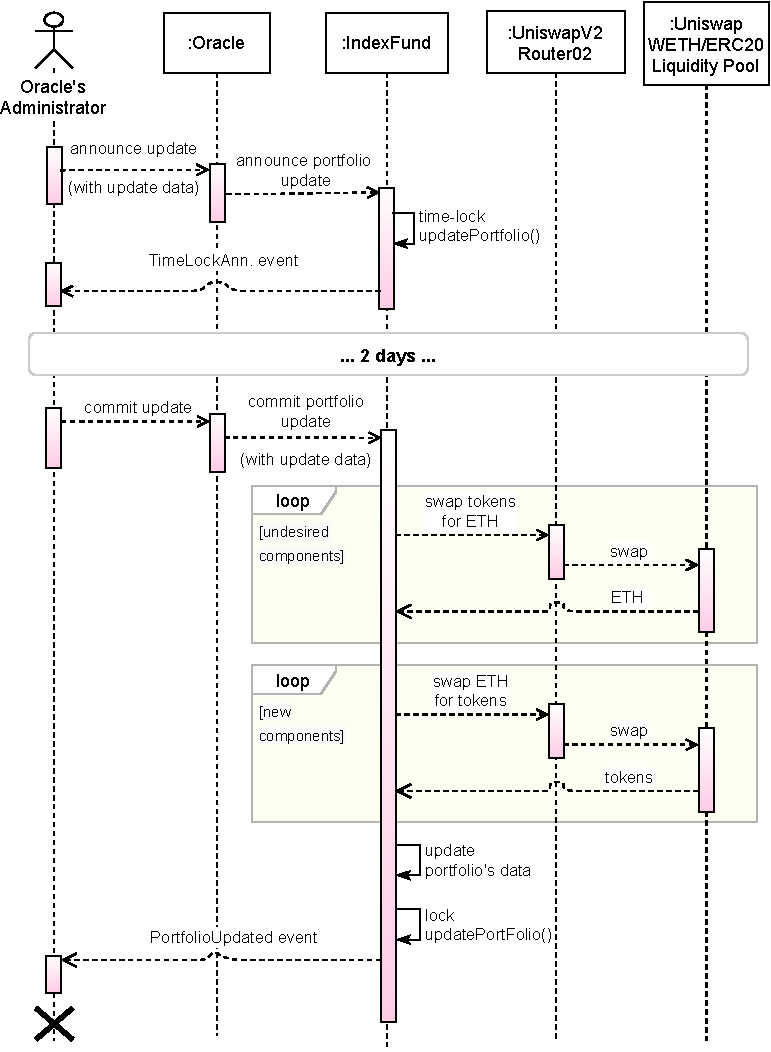
\includegraphics[width=\linewidth]{figures/update-seq.pdf}
  \caption{Portfolio update workflow of \texttt{IndexFund}}
  \label{fig:seq_update}
\end{figure}

The portfolio update functionality in the \texttt{IndexFund} contract requires the activation of time-locking on a function responsible for the process. The functions pertaining to the portfolio update process are allowed to be invoked only by the \texttt{Oracle} smart contract due to the \texttt{onlyOracle} function modifier.  
The \texttt{Oracle} contract is in turn managed by the administrator of \texttt{IndexFund}, as such, the administrator is in fact the entity executing the update process in an indirect manner through contract \texttt{Oracle}. There are three reasons for this indirect interaction between the administrator and \texttt{IndexFund}. First, contract \texttt{Oracle} is a place for serving the public inspection of the new portfolio information, especially for the investors to act appropriately on their investments during the grace period. Secondly, this can offload part of the lengthy code for the portfolio update process to another smart contract, thereby, achieving better code organization as well as reducing the code of \texttt{IndexFund} to avoid reaching the contract size limit of 24,576 bytes introduced by the EIP-170 \cite{eip170}. The final reason is to demonstrate with the system prototype the use of an oracle as means for more sophisticated data feeding such as prices from CEXs into the \texttt{IndexFund} contract in future versions of the system. From the sequence diagram in Figure \ref{fig:seq_update}, the process of updating the portfolio of \texttt{IndexFund} from \texttt{Oracle} can be visually clarified. This process is verbally dismantled in the following description for a deeper insight.

\begin{description}
  \item[Step 1: Announcing the portfolio rebalancing through the contract \texttt{Oracle}] --- The portfolio update is initiated by the administrator account of \texttt{Oracle} by sending a transaction carrying the update data to call the function \texttt{announceUpdate} in the \texttt{Oracle} contract. The update data includes the symbols of component tokens to be replaced (\texttt{\_componentsOut}), the addresses of the new tokens (\texttt{\_componentAddrsIn}), the array of all symbols for the new portfolio (\texttt{\_allNextComponents}), a set of the ITSA's International Token Identification Numbers (ITINs) corresponding to all the tokens of the new portfolio and finally, an optional announcement message from the administrator. These pieces of information will be passed to the \texttt{announceUpdate} function as function parameters and they will be stored in the respective public state variables for inspection from any interested parties. Afterwards, the function \texttt{announcePortfolioUpdating} of \texttt{IndexFund} is called from the \texttt{Oracle} contract with the announcement message as its single parameter to activate the time locking for a period of two days. At the end, the \texttt{TimeLockAnnouncement} event will be emitted from the \texttt{IndexFund} contract with the announcement and the due date of the time lock.
  
  \item[Step 2: Invoke the portfolio updates] --- When the two-day locking time has elapsed, the administrator can send another transaction to the  \texttt{Oracle} contract to invoke the \texttt{commitUpdate} function, which in turn calls the \texttt{updatePorfolio} function of \texttt{IndexFund} with all the portfolio information currently in the state variables of \texttt{Oracle}, except for the set of ITINs. Also, it should be noted that, for the purpose of front-running prevention, there are two \texttt{uint256[]} arrays passed to the \texttt{commitUpdate} function and then to the \texttt{updatePorfolio} function to specify the expected ETH outputs of the replaced tokens and the expected outputs of the new tokens for the swaps on Uniswap.
  
  \item[Step 3: Swap all the undesired components for ETH on Uniswap] ---  Based on the symbol of the to-be-replaced tokens encoded in the parameter \texttt{\_componentsOut}, the \texttt{updatePorfolio} function can look up the corresponding addresses from the current \texttt{portfolio} mapping and swap the token funds of those components for ETH on Uniswap. After each swap the respective token address is also discarded from the \texttt{portfolio} mapping to redeem the storage of the contract.
  
  \item[Step 4: Swap the received ETH for the new components] --- Due to the fact that all tokens in the portfolio are ERC20-compliant, the symbols of the new component tokens can be retrieved by calling the \texttt{symbol} function in the respective smart contracts using the contract addresses in the parameter \texttt{\_componentAddrsIn}. Then, the total amount of ETH received from Uniswap by selling the replaced tokens can now be divided evenly among the new component tokens for their purchases at the respective liquidity pools on Uniswap. 
  
  \item[Step 5: Change portfolio's components] --- In this step, the parameter \texttt{\_allNextcomponents} is assigned to the \texttt{components} state variable to replace the old set of token symbols with a new one. The reason for passing all symbols of the new portfolio instead of only the retained tokens is to avoid another loop and complicated array concatenations for assembling the array of token symbols for the new portfolio. This can potentially save some amount of gas used for the loop and reduce the complexity of smart contract code, thereby, avoiding potential bugs and enhance the security through simplicity.
  
  \item[Step 6: Lock the \texttt{updatePortfolio} function] --- As the final step, the function will lock itself for an unlimited amount of time until the next update announcement activates the time-locking period again. Finally, the \texttt{updatePortfolio} function will emit an \texttt{PortfolioUpdated} event with information about the symbols of the replaced tokens as well as the newly incoming ones.
  
\end{description}

As a result, all the funds of the substituted component tokens are sold in order to buy the funds of the new component tokens and the token information in the state variable are also appropriately replaced, thereby, the \texttt{IndexFund} contract completely removed the undesired components out of the portfolio and can continue to function with a set of better components that can potentially provide more profits for the shareholders. 
 
\subsection{Portfolio Rebalancing} \label{subsec:reblance}

In finance, rebalancing is a process of maintaining the assets in a portfolio at the weights according to a \textit{target allocation} by selling the overperforming assets and buying the underperforming ones \cite{portfoliorebalancing}. For example, if an investor set a target allocation for the total value of the portfolio at 60\% stocks and 40\% bonds, then an increase in stock price will cause the weighting of stocks and bonds to deviate from this 60/40 allocation, therefore, the investor should then sell some stocks and buy some bonds to rebalance the portfolio back to target allocation. The purpose of the portfolio rebalancing process is to preserve the investment goals and ensure that the amount of financial risks is maintained within the tolerance of the investor. 

The concept of rebalancing can also be applied to the portfolio of our decentralized index fund. For this purpose, the \texttt{IndexFund} contract provides a public function \texttt{rebalance} that can only be invoked from the \texttt{Oracle} contract to perform the portfolio rebalancing with a fixed, uniform target allocation among the component tokens. 
In our design, the portfolio rebalancing is in fact initiated by the administrator (or the owner) of the \texttt{Oracle} contract, which in turn activates the grace period of two days on the \texttt{rebalance} function. After that period of time, the \texttt{Oracle} contract can invoke the \texttt{rebalance} function to effectively perform the portfolio rebalancing. This behavior of time-locking activation from the \texttt{Oracle} contract is similar to that of the periodic portfolio update described earlier. Nonetheless, The complete rebalancing process can be explained in detail as follows.


% Note that from this point onward, for the sake of brevity, we will prefix the name of functions with the name of the contract it resides in and separate the two names by a dot, e.g., \texttt{IndexFund.rebalance()} indicates the \texttt{reblance} function in the \texttt{IndexFund} contract. With that in mind, the 

\begin{description}
  \item[Step 1: Announce the portfolio rebalancing through the \texttt{Oracle} contract] ---  Before the portfolio rebalancing process can be performed, it is required that the function responsible for this process in the \texttt{IndexFund} contract is applied a lock time of two days, during which that function cannot be executed. This lock time is a grace period for investors to redeem their investments if they disagree with the upcoming rebalancing. Also, only the \texttt{Oracle} contract can activate this lock time, and in turn, only the administrator of \texttt{Oracle} can initiate the call from \texttt{Oracle} to \texttt{IndexFund} to time-lock that function. The goal of this step is not only to time-lock the \texttt{rebalance} function in \texttt{IndexFund}, but also to announce the portfolio rebalancing to interested parties through an event emitted at the end.
  
  
  \item[Step 2: Execute the rebalancing] --- After the grace period of two days, the administrator of \texttt{Oracle} again invokes an intermediary function in the \texttt{Oracle} contract to ultimately call the \texttt{rebalance} function in the \texttt{IndexFund} contract to perform the rebalancing. For the sake of simplicity in the context of a system prototype, we apply a uniform weights to every component tokens, meaning \texttt{IndexFund} should maintain the same ETH net asset value (NAV) for each individual token in the portfolio, thus the target allocation of our rebalancing is a uniform one. Through the Uniswap router contract, the \texttt{rebalance} function can assess the total NAV of all component tokens of \texttt{IndexFund}. The total sum of NAV will be divided by the number of components in the portfolio (the portfolio size) to obtain the average NAV, at which the NAV of each component should be maintained to respect the uniform weights. For a component token with NAV exceeding the average NAV, a portion of its amount will be swapped on Uniswap for ETH to reduced its NAV to the average NAV assessed earlier. Then, the amount of ETH received from Uniswap can be swapped again on Uniswap for the component tokens with their NAV less than the average ETH value so that their NAV is raised to the average. As a result, by selling the overperforming tokens and buying the underperforming ones in term of their NAV with respect to the average NAV of the whole portfolio, all component tokens will have approximately the same NAV after the rebalancing. 
  
  \item[Step 3: Lock the \texttt{rebalance} function] --- At the end, the \texttt{rebalance} function will lock itself for an indefinite amount of time until the time lock of two days is activated again through the \texttt{Oracle} contract. In addition, an event is emitted to inform the interested parties about the occurrence of the rebalancing.
\end{description}



\section{The Oracle Infrastructure} \label{sec:oracleinfras}

Through the process of updating the portfolio in section \ref{subsec:updateportfolio}, the roles and functionalities of the oracle infrastructure have been more or less exposed. This section aims to describe the oracle components in a definitive manner with clear description of their roles in the system. As shown in Figure \ref{fig:sys_architecture} of system architecture, the oracle infrastructure consists of an on-chain and an off-chain components. The on-chain component is a smart contract, while the off-chain component can be one or more oracle nodes interacting directly with the oracle smart contract on the blockchain. Together, they perform the task of feeding external data from the world outside Ethereum onto the blockchain.

Our oracle infrastructure in this prototype follows both the Intermediate-Read as well as Publish-Subscribe oracle patterns discussed in section \ref{subsubsec:background_oracle}. The reason for being an Intermediate-Read oracle is that our oracle contract receives data from oracle node not frequently, although periodically, to serve data lookup from the interest Ethereum participants. On the other hand, the Publish-Subscribe is attributed by the fact that the portfolio information used for the update is \textit{pushed} from the oracle contract to its client, which is the \texttt{IndexFund} smart contract. As a result, our oracle infrastructure do not strictly follow any single oracle pattern but rather combine both of the two aforementioned ones. In the following, we dismantle our oracle infrastructure by its on-chain and off-chain components and discuss their respective roles and functionalities in the specific context of our decentralized index fund.

\subsection{Oracle Contract}

The oracle contract in our system is named \texttt{Oracle} and acts as an intermediator between its administrator and the \texttt{IndexFund} contract during both the portfolio update and rebalancing processes. Therefore, this on-chain oracle component interacts directly with the \texttt{IndexFund} contract on the blockchain and receives extrinsic data from the off-chain oracle node managed by the oracle administrator. 
The structure of the \texttt{Oracle} contract is outlined in Listing \ref{lst:oracle} with the set of state variables as well as the two important function used in the portfolio update workflow in Figure \ref{fig:seq_update}. In general, the \texttt{Oracle} contract is quite short since it is supposed to be a transient data storage for the portfolio update process and offloads only a part of the code for portfolio update process. However, if the \texttt{IndexFund} contract is extended with more features requiring more external data, the Oracle contract might be also extended in tandem to carry more data and offload more code for \texttt{IndexFund}. It should be noted that the code shown in Listing \ref{lst:oracle} is not the complete code of the \texttt{Oracle} smart contract with the ellipses (\dots) indicating the omission of some code snippets not shown for the sake of brevity and emphasis of the important parts of the smart contract.  

\begin{lstlisting}[language=Solidity, label={lst:oracle}, captionpos=b, caption={Partial Solodity code of the \texttt{Oracle} contract}]
contract Oracle is Ownable {
    address payable public indexFund;

    string[] public componentsOut;
    address[] public componentAddrsIn;
    string[] public allNextComponents;
    string[] public componentITINs;
    
    function announceUpdate(
        string[] memory _componentsOut, address[] memory _componentAddrsIn, 
        string[] memory _allNextcomponents, string[] memory _componentITINs, 
        string calldata _announcementMessage
    ) external onlyOwner 
    {
        ...
        IndexFund(indexFund).announcePortfolioUpdating(_announcementMessage);
    }

    function commitUpdate(
        uint256[] calldata _amountsOutMinOut, uint256[] calldata _amountsOutMinIn
    ) external onlyOwner 
    {
        IndexFund(indexFund).updatePorfolio(
            componentsOut, _amountsOutMinOut, 
            componentAddrsIn, _amountsOutMinIn, 
            allNextcomponents
        );
    }
    ...
}
\end{lstlisting}

With the function modifiers \texttt{onlyOwner} marked on the functions \texttt{announceUpdate} and \texttt{commitUpdate}, which are the functions relevant for the portfolio update process, we ensure that the administrator (or the owner) of \texttt{Oracle} is the only entity that can initiate and perform the portfolio update. To start the update, the administrator calls the \texttt{announceUpdate} function and uploads the external data through the function parameters. Except for \texttt{\_announcementMessage}, the other array parameters are assigned to the respective public state variables in the function body and afterwards, the function \texttt{announcePortfolioUpdating} of \texttt{IndexFund} is invoked with the announcement to activate the grace period of two days for the \texttt{updatePortfolio} function in \texttt{IndexFund}. During this grace period, the administrator is not able to run the \texttt{commitUpdate} function from lines 19 to 28 since the call \texttt{IndexFund(indexFund).updatePorfolio(...)} will fail due to the ongoing grace period. Therefore, with the lock time applied, the order "first \textit{announce} then \textit{commit}" is enforced and administrator cannot perform otherwise. In this manner, the investors are assured that their investments are safe against potential scams or frauds since they will always have a grace period of two days to inspect the new portfolio information from \texttt{Oracle} and make decisions upon their current investments before the update is actually executed with the administrator calling the \texttt{commitUpdate} function. The contents of the update data incorporated into the state variables through the \texttt{announceUpdate} function that can be inspected by any interested parties are following:

\begin{itemize}
    \item \texttt{componentsOut} --- This variable is a string array storing the symbols of the outgoing/to-be-replaced/undesired components tokens, whose contract addresses can be the looked up in the \texttt{portfolio} mapping of contract \texttt{IndexFund}.
    
    \item \texttt{componentAddrsIn} --- This holds the Ethereum addresses of the incoming/new component tokens, whose symbols can then be retrieved with the \texttt{symbol} function of the ERC20's interface since the tokens are required to be ERC20-compliant to become part of the portfolio.
    
    \item \texttt{allNextcomponents} --- This variable contains all the symbols of component tokens for the next portfolio after the update. This array of token symbols is supposed to replace the entire \texttt{components} array state variable in the \texttt{IndexFund} contract. Therefore, symbols of the retained tokens in the portfolio are also part of this array for the purpose of avoiding the involved operations on arrays to filter and incorporate the retained token components into the new portfolio.
    
    \item \texttt{componentITINs} --- The ITINs of the tokens in the new portfolio are included in this variable with the their order according to the respective symbols in \texttt{allNextcomponents}. Even though this array of ITINs will not be pushed to the \texttt{IndexFund} contract as with the other three array state variables, they support the inspectors in the validation of the token symbols because ITINs are the numbers uniquely identifying every token in the cryptocurrency world, while token symbols can possibly be duplicated, although this is rarely the case. Even after a portfolio update has been completed, the ITINs are still available until the next update is initiated, thus, any interested parties can always perform cross-validation of token information from the ITSA's API using the ITINs stored in this state variable to ensure the portfolio consists of the correct component tokens. In future versions of the system when the ITINs becomes more popular, it is possible and also trivial to completely represent the component tokens in the \texttt{IndexFund} contract by their ITINs in place of their symbols since they are both string arrays.
    
\end{itemize}

By default, Solidity will create for each state variable marked as \texttt{public} a getter function with exact same name. However, for array type, its default getter function requires an array index as parameter and can return only a single element at that index instead of the whole underlying array. Thus, the \texttt{Oracle} contract in fact also provides a set of custom getter functions, e.g., \texttt{getcomponentsOut}, that can return the an entire respective array for the purpose of easing the inspection of the update data. In addition, there is a getter function for viewing the end time of the \texttt{updatePortfolio} function of \texttt{IndexFund}. Finally, the two functions \texttt{announceRebalancing} and \texttt{commitRebalancing} pertaining to the rebalancing process are not guarded by the \texttt{onlyOwner} modifier and support the same principle "first \textit{announce} then \textit{commit}" as their counterparts for the portfolio update process.

\subsection{Oracle Node} \label{subsec:oracle_node}

In our system, we assume that the oracle node is represented by the single EOA of the administrator and can be realized by one or many machines irrespective of their geographic locations. As such, anyone with access to the private key of the administrator EOA can act as the oracle node, especially when the administrator is the representation of an organization on the Ethereum network. Therefore, the noun phrase "oracle node" in singular form that we have been using throughout this paper indeed indicates the off-chain component of the oracle infrastructure, although this component can comprise multiple machines. Also, for the sake of simplicity within the scope of a system prototype, we only have one EOA acting as the administrator of the entire on-chain subsystem and thus, the oracle node can also be deemed as an Ethereum node, which is represented by an EOA as clarified in the Background section. However, if the \texttt{Oracle} contract should be governed by multiple EOAs in the future, the meaning of "oracle node" is only the off-chain component of the infrastructure.

In general, the main task of an oracle node is collecting data from the outside world and feeding it to the Ethereum network to address the restriction of the EVM not allowing smart contracts to communicate with external data sources for the purpose of preserving the  state transition determinism required by the consensus protocol. In our system, the oracle node also has the responsibility of selecting the component tokens for the portfolio in addition to retrieving token data from the ITSA's API and transmitting it to the \texttt{Oracle} contract on the blockchain. Specifically, these responsibilities can be characterized as follow.

\begin{description}
  \item[Retrieve token information from ITSA] --- Due to the requirement that our token portfolio should follow the tokens in a specific category, the oracle node has the responsibility for obtaining the classified token data from the ITSA database in order to correctly select the tokens with that same category for the section of new components during the portfolio update. 
  
  \item[Select component tokens for the portfolio] --- The task of selecting an optimal portfolio is a mathematically complicated task and thus, is beyond the scope of this thesis. Therefore, we use employ an very simple heuristic for this task on the oracle node to test the functionality of the oracle infrastructure. For each update, the oracle node will store the Uniswap pools' price of all candidate tokens that satisfy the category of the portfolio. Then, During a portfolio update, the token prices will be compared to their counterparts in the last update and tokens that perform better will have the higher chance to become the next portfolio's components, while the current components, which perform worse than the last time, will be pushed out of the portfolio. This heuristic is quite naive and does not guarantee to select the optimal set of components, however, it is sufficient to test for the functioning of the oracle node in the scope of a system prototype.
  
  \item[Upload data to the \texttt{Oracle} contract] --- Once the new set of components for the portfolio is selected and an update to the portfolio is required, the oracle node can then upload the data of the new portfolio to the \texttt{Oracle} contract for public inspection before this data effectively replaces the data of the current portfolio in the \texttt{IndexFund} contract.
  
\end{description}


\section{Client Application}  \label{sec:cli}

Technically, any programs or libraries with the ability to send transactions to the Ethereum blockchain can in fact become the client of our DeFi application. For example, we utilize Remix IDE to communicate with the \texttt{Indexfund} and \texttt{Oracle} contracts deployed on the Ropsten testnet as described in section \ref{sec:ropsten_tesnet}.

As a client application is an optional requirement for our system prototype, we have prepared a test set to ensure the functionalities of this DeFi application, therefore, we could put more focus on other more important parts of the system during the course of the thesis. However, we still plan to have a graphical user interface for the prototype in the near future, especially for the demonstration of the prototype during the defence of this thesis.